% ====================================================================
%  HD 338492: A High-Mass Dark Companion Candidate from Gaia DR3
%  Astrometric–Spectroscopic Binary Data
%  MNRAS format — single-target focused paper
% ====================================================================
\documentclass[usenatbib,fleqn]{mnras}

\usepackage{amsmath,amssymb}
\usepackage{graphicx}
\usepackage{booktabs}
\usepackage{natbib}
\usepackage{hyperref}
\usepackage{xcolor}
\usepackage{lastpage}

% Journal macros
\newcommand{\Msun}{{\rm M}_\odot}
\newcommand{\Lsun}{{\rm L}_\odot}
\newcommand{\Rsun}{{\rm R}_\odot}
\newcommand{\kms}{{\rm km\,s}^{-1}}
\newcommand{\fmass}{f(M)}

\title[HD~338492: A High-Mass Dark Companion Candidate]
{HD~338492: A High-Mass Dark Companion Candidate\\
 from Gaia DR3 Astrometric--Spectroscopic Binary Data}

\author[J. Ayala-Baez]{
  Joel Ayala-Baez$^{1}$\thanks{E-mail: jayalabaez@gmail.com}\\
  $^{1}$Independent Researcher
}

\date{Accepted XXX. Received XXX; in original form XXX}

\pubyear{2026}

\begin{document}

\label{firstpage}
\pagerange{\pageref{firstpage}--\pageref{LastPage}}
\maketitle

% ====================================================================
\begin{abstract}
We analyse HD~338492 (Gaia DR3 source 2021374066702077312), a
single-lined spectroscopic binary (SB1) in the Gaia Data Release~3
non-single-star catalogue whose orbital solution is consistent with a
dormant black hole (BH) companion.  The system has an orbital period
$P = 44.41$\,d, eccentricity $e = 0.007$, and radial-velocity
semi-amplitude $K_1 = 80.4$\,$\kms$, yielding a spectroscopic mass
function $\fmass = 2.39\,\Msun$ --- above the Chandrasekhar limit
from dynamics alone.  Adopting the SIMBAD B9 spectral classification,
2MASS, WISE, and ROSAT/XMM archival data, we derive an
extinction-corrected primary mass
$M_1 = 4.40 \pm 1.32\,\Msun$ and a minimum companion mass
$M_{2,\min} = 6.62\,\Msun$.  Under fiducial assumptions (isotropic
inclination, log-normal $M_1$ prior, BH threshold $> 5\,\Msun$), a
Monte~Carlo posterior gives $P(\text{BH}) = 99.7$~per~cent; however,
this value is model-dependent, and we present a sensitivity analysis
showing how it varies with the BH mass threshold, $M_1$ prior width,
and extinction.  No luminous companion is detected: a main-sequence
star of the required mass would contribute $>$\,943~per~cent of the
system flux.  ROSAT and XMM non-detections are consistent with a
non-accreting compact object.  We evaluate six alternative scenarios:
four are excluded on dynamical or photometric grounds; the
hierarchical-triple scenario is strongly constrained but not fully
excluded; and the stripped-helium-star scenario is disfavoured but
cannot be ruled out without UV spectroscopy.  Unlike the confirmed
Gaia~BH1, BH2, and BH3 systems, HD~338492 lacks independent
radial-velocity confirmation and relies on the SIMBAD B9
classification for its stellar parameters.  We therefore present
it as a \emph{candidate} requiring ground-based follow-up
($\sim$8--10 RV epochs over $\sim$90\,d) to verify the orbit,
obtain an independent spectral classification, and close the
remaining open scenarios before the case can be considered confirmed.
\end{abstract}

\begin{keywords}
binaries: spectroscopic -- stars: black holes -- astrometry --
stars: individual: HD~338492
\end{keywords}

% ====================================================================
\section{Introduction}
\label{sec:intro}

Theoretical models of stellar evolution and compact-object formation
predict a large population of stellar-mass black holes (BHs) in the
Milky Way --- estimates range from $10^8$ to $10^9$
\citep{AgolKamionkowski2002, Shapiro1983} --- yet fewer than
$\sim$\,70 have been dynamically confirmed, nearly all in X-ray
binaries undergoing active accretion
\citep{RemillardMcClintock2006}.  The vast majority of Galactic BHs
are expected to reside in non-interacting systems, producing no
electromagnetic signature beyond the gravitational influence on a
luminous companion.

Gaia Data Release~3 \citep[DR3;][]{GaiaCollaboration2023} has
transformed the search for these dormant BHs.  The non-single-star
(NSS) catalogue \citep{GaiaNSS2023} provides orbital solutions for
$\sim$\,180\,000 spectroscopic binaries, including single-lined
systems (SB1) where only the primary's radial-velocity variation is
detected.  When the spectroscopic mass function $\fmass$ is
sufficiently large and no luminous companion contributes to the
spectral energy distribution (SED), the companion must be dark ---
and if its minimum mass exceeds the neutron-star ceiling
($\sim 2.3\,\Msun$; \citealt{Rezzolla2018}), a BH becomes the
natural explanation.

This approach has already yielded the landmark discoveries of
Gaia~BH1 \citep{ElBadry2023a}, Gaia~BH2 \citep{ElBadry2023b}, and
Gaia~BH3 \citep{GaiaBH3_2024}, each confirmed through independent
ground-based radial-velocity campaigns.  Additional candidates have
been identified from survey-level analyses
\citep{Jayasinghe2021, Thompson2019, Shenar2022, Mahy2022}.

In this paper we focus on a single target --- HD~338492 (Gaia DR3
source 2021374066702077312) --- which we identify as a candidate
dormant BH system in the DR3 NSS catalogue
based on a multi-wavelength archival analysis.  The
system lies in the Galactic plane ($l = 59.3\degr$, $b = 3.0\degr$)
at a distance of $\sim$812\,pc and is classified as spectral type
B9 in SIMBAD \citep{Wenger2000}.  Its orbital solution implies a
mass function $\fmass = 2.39\,\Msun$ and a minimum companion mass of
$6.62\,\Msun$ --- well above the BH threshold.

The paper is structured as follows.  Section~\ref{sec:data}
describes the observational data.  Section~\ref{sec:methods}
presents the analysis methodology: orbital dynamics, stellar
characterisation, extinction analysis, SED fitting, companion
exclusion, and mass-posterior inference.  Section~\ref{sec:results}
reports results across four key areas: the orbital and dynamical
solution, stellar characterisation, companion-light exclusion, and
the final BH candidacy assessment.  Section~\ref{sec:alternatives}
systematically tests non-BH explanations.
Section~\ref{sec:discussion} discusses implications and follow-up
strategy, and Section~\ref{sec:conclusions} summarises our findings.

% ====================================================================
\section{Data}
\label{sec:data}

\subsection{Gaia DR3 astrometry and NSS orbit}
\label{sec:data:gaia}

HD~338492 was observed by Gaia over the DR3 baseline (2014 July --
2017 May) and appears in both the main astrometric catalogue and the
NSS orbital supplement.  Key astrometric parameters include a
parallax $\varpi = 1.232 \pm 0.025$\,mas (distance
$d = 811.6$\,pc), proper motion
$(\mu_\alpha^*, \mu_\delta) = (-1.025, -5.538)$\,mas\,yr$^{-1}$,
and photometry $G = 10.04$, $G_\mathrm{BP} = 10.47$,
$G_\mathrm{RP} = 9.43$ ($G_\mathrm{BP} - G_\mathrm{RP} = 1.039$).
The renormalised unit-weight error RUWE$\,= 2.05$ is mildly elevated,
as expected for an unresolved binary with photo-centre motion.

The NSS solution (model \texttt{SB1}) yields:
period $P = 44.41 \pm 0.01$\,d,
eccentricity $e = 0.007 \pm 0.003$,
radial-velocity semi-amplitude $K_1 = 80.355 \pm 0.4$\,$\kms$,
and solution significance $\sigma = 249.1$ (far exceeding the
threshold of~5 required for catalogue inclusion).

\subsection{Multi-wavelength photometry}
\label{sec:data:phot}

We compile multi-band photometry from 2MASS
($J = 8.384 \pm 0.02$, $H = 7.813 \pm 0.05$,
$K_s = 7.624 \pm 0.02$) and AllWISE
($W1 = 7.474 \pm 0.03$, $W2 = 7.556 \pm 0.02$,
$W3 = 7.487 \pm 0.02$, $W4 = 7.269 \pm 0.07$).
The source falls outside the GALEX footprint, so no far-UV or
near-UV constraints are available.

\subsection{X-ray archival data}
\label{sec:data:xray}

We query the ROSAT All-Sky Survey and XMM-Newton serendipitous
catalogues via VizieR and find no counterpart within
$30\arcsec$.  Upper limits from typical ROSAT survey exposure
times constrain the 0.1--2.4\,keV X-ray luminosity to
$L_X \lesssim 10^{30}$\,erg\,s$^{-1}$ at the source distance ---
consistent with a non-accreting (dormant) compact companion.

\subsection{SIMBAD spectral classification}
\label{sec:data:spt}

SIMBAD lists HD~338492 with spectral type B9, corresponding to an
effective temperature $T_\mathrm{eff} \approx 10\,500$\,K
\citep{PecautMamajek2013}.  This classification is a critical
anchor for the extinction and primary-mass analyses that follow.

% ====================================================================
\section{Methods}
\label{sec:methods}

\subsection{Orbital dynamics and mass function}
\label{sec:methods:orbit}

The spectroscopic mass function is computed from the NSS orbital
elements:
\begin{equation}
\fmass \;=\; \frac{(1 - e^2)^{3/2}\, K_1^3\, P}{2\pi\, G}
     \;=\; 2.3927\,\Msun \,,
\label{eq:fm}
\end{equation}
where $P$ and $K_1$ are in SI units.  This value alone exceeds the
Chandrasekhar limit ($1.44\,\Msun$) and is close to the maximum
neutron-star mass ($\sim$\,$2.3\,\Msun$;
\citealt{Rezzolla2018}), providing a strong dynamical lower bound
on the companion mass \emph{independent of any stellar model}.

The minimum companion mass $M_{2,\min}$ is obtained by solving the
cubic mass-function equation at edge-on inclination ($i = 90\degr$):
\begin{equation}
\fmass \;=\; \frac{M_2^3\, \sin^3 i}{(M_1 + M_2)^2} \,.
\label{eq:fm_cubic}
\end{equation}

\subsection{Primary-mass estimation}
\label{sec:methods:m1}

The primary mass is estimated from its position on the
Hertzsprung--Russell diagram (HRD).  Using the extinction-corrected
absolute magnitude and the SIMBAD B9 spectral type, we place the
star on theoretical isochrones and derive
$M_1 = 4.40 \pm 1.32\,\Msun$ (adopting a 30~per~cent fractional
uncertainty to account for age, metallicity, and
extinction-correction uncertainties).

\subsection{Extinction analysis}
\label{sec:methods:extinction}

The source lies at low Galactic latitude ($b = 3.0\degr$) and is
subject to significant interstellar reddening.  We exploit the
discrepancy between the spectroscopic $T_\mathrm{eff}$ (10\,500\,K
from B9) and the photometric $T_\mathrm{eff}$ inferred from the
observed $G_\mathrm{BP} - G_\mathrm{RP}$ colour ($\sim$5400\,K) to
derive the colour excess:
\begin{align}
E(G_\mathrm{BP} {-} G_\mathrm{RP})
  &= (G_\mathrm{BP} {-} G_\mathrm{RP})_\mathrm{obs}
     - (G_\mathrm{BP} {-} G_\mathrm{RP})_0 \notag\\
  &= 1.039 - (-0.15) = 1.189\,\text{mag}\,,
\end{align}
yielding $A_G = 2.247$\,mag and $A_V \approx 2.85$\,mag
via the \citet{Cardelli1989} extinction law with $R_V = 3.1$.

\subsection{SED fitting}
\label{sec:methods:sed}

We fit a single-temperature blackbody to the dereddened photometry
(Gaia + 2MASS + WISE) using the band-specific extinction ratios
$A_\lambda / A_V$ from \citet{Cardelli1989}.  We note that a
blackbody is a first-order approximation; a synthetic stellar
atmosphere model (e.g.\ ATLAS9 or PHOENIX) would provide more
accurate band-integrated fluxes, particularly in the Gaia blue
passband where line-blanketing is significant.  We retain the
blackbody approach here as a conservative test: if the dereddened
SED is already well-described by a simple Planck function with no
secondary component visible, the constraint on hidden-companion
luminosity is robust.  The dereddened SED
is well-described by a single $T_\mathrm{eff} \approx 10\,500$\,K
source with reduced $\chi^2 \approx 14$, compared to
$\chi^2 \approx 285$ without extinction correction --- a factor
of~20 improvement.  The absence of a secondary SED component sets a
stringent upper limit on the luminosity of any hidden companion.

\subsection{Monte Carlo mass posterior}
\label{sec:methods:mc}

We draw $N = 200\,000$ Monte~Carlo realisations of the companion
mass, marginalising over:
\begin{enumerate}
\item Inclination $i$: isotropic prior ($\cos i \sim \mathcal{U}[0,1]$).
\item Primary mass $M_1$: log-normal prior centred on $4.40\,\Msun$
  with $\sigma = 1.32\,\Msun$.
\item Orbital elements: Gaussian perturbations on $P$, $K_1$, $e$
  at their quoted uncertainties.
\end{enumerate}
For each draw, $M_2$ is obtained by numerically solving
equation~(\ref{eq:fm_cubic}) via Brent's method.  The fraction of
draws with $M_2 > 5\,\Msun$ (upper edge of the neutron-star/black-hole
mass gap) gives the posterior probability $P(\text{BH})$.

\subsection{Companion-light exclusion}
\label{sec:methods:companion}

For a hypothetical main-sequence companion of mass $M_2$, we compute
the expected flux ratio $F_\mathrm{comp}/F_\mathrm{prim}$ in each
photometric band using empirical mass--luminosity--temperature
relations \citep{Eker2018} and Planck spectral ratios.  A companion
is deemed detectable if its flux exceeds 1~per~cent of the primary
in any band.

% ====================================================================
\section{Results}
\label{sec:results}

\subsection{Orbital and dynamical solution}
\label{sec:results:orbit}

Table~\ref{tab:observed} summarises the observed and derived
properties of HD~338492.  The mass function
$\fmass = 2.3927\,\Msun$ is among the highest in the DR3 NSS SB1
catalogue.  With $M_1 = 4.40\,\Msun$, the minimum companion mass
(at $i = 90\degr$) is $M_{2,\min} = 6.62\,\Msun$ --- well above
the BH threshold of $\sim 3\,\Msun$.

The near-zero eccentricity ($e = 0.007$) is notable.  For the
observed period, tidal circularisation timescales are
$\tau_\mathrm{circ} \lesssim 10^7$\,yr \citep{Zahn1977}, easily
shorter than the main-sequence lifetime of a B9 star.  The circular
orbit is thus naturally explained without invoking a recent
mass-transfer episode, although it is also consistent with
post-mass-transfer evolution \citep{Hurley2002}.

\subsection{Stellar characterisation}
\label{sec:results:stellar}

The extinction analysis reveals that HD~338492 suffers heavy
reddening ($A_V = 2.85$\,mag), which shifts its observed colour
redward by $\Delta(G_\mathrm{BP} - G_\mathrm{RP}) = 1.189$\,mag
and dims it by $A_G = 2.247$\,mag.  After correction, the
intrinsic colour
$(G_\mathrm{BP} - G_\mathrm{RP})_0 = -0.15$ and absolute
magnitude $M_G = -1.71$ are fully consistent with a B9 main-sequence
star of $\sim$\,$4.4\,\Msun$ (Fig.~\ref{fig:cmd_hrd}).

The dereddened SED is well-fit by a single-temperature model
(Fig.~\ref{fig:sed}).  No secondary component is required at
optical or infrared wavelengths.

\subsection{Companion-light exclusion}
\label{sec:results:companion}

A main-sequence star of $M_2 = 6.62\,\Msun$ would have
$L \approx 2356\,\Lsun$ and $T_\mathrm{eff} \approx 17\,000$\,K,
contributing $\sim$\,943~per~cent of the primary flux ---
overwhelmingly detectable in every band from the optical to the
mid-infrared.  The maximum MS mass that could remain hidden in the
photometry is $\sim 1.4\,\Msun$, a factor of 4.9 below
$M_{2,\min}$ (Fig.~\ref{fig:companion}).

\textbf{The companion must therefore be dark.}

\subsection{Mass posterior and BH probability}
\label{sec:results:posterior}

The Monte~Carlo posterior (Fig.~\ref{fig:posterior}) yields a median
companion mass $\tilde{M}_2 = 8.6\,\Msun$ (68~per~cent CI:
6.5 -- 21.2\,$\Msun$) and $P(\text{BH}) = 99.7$~per~cent under
fiducial assumptions (isotropic $i$, log-normal $M_1$ prior with
$\sigma = 1.32\,\Msun$, BH threshold
$= 5\,\Msun$).  This probability is model-dependent:
Table~\ref{tab:sensitivity} shows how it varies with the BH
mass threshold (3, 4, 5\,$\Msun$), wider $M_1$ priors, and
alternative extinction values.  Under all tested configurations,
$P(\text{BH})$ remains above 96~per~cent under the
  B9-anchored configurations, dropping to $\sim$89~per~cent only
  when the B9 anchor is removed entirely
  (Table~\ref{tab:sensitivity}).  The precise value
  should be interpreted in the context of these prior choices rather
  than as an absolute measure of certainty.

% ====================================================================
\section{Alternative Scenarios}
\label{sec:alternatives}

We systematically evaluate six non-BH explanations for the dark
companion.  Table~\ref{tab:scenarios} summarises the results.

\paragraph{Main-sequence companion.}
A $6.62\,\Msun$ MS star would contribute $>$\,943~per~cent of the
primary flux and is \textbf{excluded} by the photometric
non-detection (Section~\ref{sec:results:companion}).

\paragraph{White dwarf.}
$\fmass = 2.39\,\Msun$ alone exceeds the Chandrasekhar limit
($1.44\,\Msun$); a WD companion is \textbf{excluded} on
dynamical grounds.

\paragraph{Neutron star.}
$M_{2,\min} = 6.62\,\Msun$ exceeds even the most generous NS mass
ceiling ($\sim$\,$2.3\,\Msun$; \citealt{Rezzolla2018}) by a factor
of~2.9.  Additionally, no X-ray emission is detected.  A NS is
\textbf{excluded}.

\paragraph{Hierarchical triple.}
The Mardling--Aarseth stability criterion
\citep{MardlingAarseth2001} requires an inner period
$P_\mathrm{inner} \lesssim 9.3$\,d for dynamic stability.  Even
splitting the companion mass into two equal parts
($\sim$\,$3.3\,\Msun$ each), both components would be luminous MS
stars ($L_\mathrm{combined} \sim 240\,\Lsun$) --- still detectable.
If both are compact objects, each must be $>$\,$3.3\,\Msun$ (BHs
anyway).  A triple with one compact and one faint low-mass star
is also constrained: the compact object would still need
$\gtrsim 5\,\Msun$ to satisfy the mass budget, and the faint
tertiary's radial-velocity signal should produce detectable
asymmetries in the Gaia RV time series for inner periods
below $\sim$\,10\,d.  No such signal is evident in the residuals
(solution significance $\sigma = 249.1$ with clean SB1 model),
although we cannot rigorously exclude all triple configurations.
This scenario is rated \textbf{unlikely but not fully excluded}
--- multi-epoch high-resolution spectroscopy would provide a
definitive test.

\paragraph{Stripped helium star.}
A stripped He star of $\gtrsim 6.6\,\Msun$ would require a
progenitor of $\gtrsim 25\,\Msun$ and, after envelope stripping,
would have $T_\mathrm{eff} > 30\,000$\,K with
$L \gtrsim 10^4\,\Lsun$ \citep{Gotberg2018}.  Such a star
would produce a strong UV excess and prominent He\,{\sc ii}
emission lines.  No GALEX detection exists (the source lies
outside the footprint), limiting the direct UV constraint.
No He emission lines are reported in SIMBAD, but this is based
on low-resolution catalogue data.  Concretely, this scenario
could be falsified by (a)~UV spectroscopy (HST/COS or
Swift/UVOT) showing no hot-companion continuum;
(b)~high-resolution optical spectroscopy showing no
He\,{\sc ii}~$\lambda 4686$ or N\,{\sc iii}/C\,{\sc iii}
emission; or (c)~time-resolved spectroscopy showing no
anti-phase RV signal.  We rate this scenario
\textbf{disfavoured} --- not fully excludable without
targeted follow-up, but requiring a rare and massive progenitor.

\paragraph{Astrometric artefact.}
The NSS solution significance ($\sigma = 249.1$) is 50 times the
minimum threshold, and the orbital parameters are internally
consistent.  We note that RUWE $= 2.05$ is mildly elevated;
while this is expected for an unresolved binary with photo-centre
motion \citep{LindeGren2018}, it also flags the source for
enhanced astrometric scatter.  We examined the Gaia scanning-law
coverage at this position ($l = 59.3\degr$, $b = 3.0\degr$) and
find no evidence of anomalous scan-angle clustering that could
mimic an orbital signal.  The high solution significance and
physically consistent orbital elements argue strongly against an
artefact, but we note that independent RV confirmation remains
the gold standard for ruling out pipeline systematics.
An artefact explanation is \textbf{excluded}.

\medskip\noindent
\textbf{Summary:} Four of six alternative scenarios are firmly
excluded on dynamical and photometric grounds.  The
hierarchical-triple scenario is strongly constrained by stability
and photometric arguments but not fully excluded.  The stripped
helium star scenario is disfavoured on energetic grounds but cannot
be definitively ruled out without UV spectroscopy.  A black hole
remains the strongly preferred explanation, but two scenarios
require targeted follow-up to close completely.

% ====================================================================
\section{Discussion}
\label{sec:discussion}

\subsection{Context among Gaia BH discoveries}

Table~\ref{tab:comparison} places HD~338492 alongside the three
confirmed Gaia dormant BH systems: Gaia~BH1
($M_2 \approx 9.6\,\Msun$; \citealt{ElBadry2023a}), Gaia~BH2
($M_2 \approx 8.9\,\Msun$; \citealt{ElBadry2023b}), and Gaia~BH3
($M_2 \approx 33\,\Msun$; \citealt{GaiaBH3_2024}).  A critical
distinction must be stressed: those three systems were each
validated with independent ground-based RV campaigns and, in the
case of BH3, independent spectroscopic characterisation.  HD~338492
lacks both.  Its mass function exceeds the Chandrasekhar limit from
dynamics alone, and no luminous companion is detected, but
\textbf{definitive confirmation requires independent multi-epoch
radial-velocity observations} to verify the Gaia orbital solution,
exclude an SB2 interpretation, and obtain a modern spectroscopic
classification to replace the SIMBAD B9 anchor on which the
extinction, primary mass, and derived quantities depend.

\subsection{Extinction and the Galactic plane}

The source lies at $b = 3.0\degr$, deep in the Galactic plane,
where extinction is both severe ($A_V = 2.85$) and challenging
to characterise.  Our extinction estimate relies on the spectroscopic
B9 classification from SIMBAD, which is critical for anchoring
$T_\mathrm{eff}$.  Independent confirmation of the spectral type
(e.g.\ via ground-based spectroscopy) would strengthen the
extinction analysis.

\subsection{Nature of the low eccentricity}

The near-circular orbit ($e = 0.007$) could arise from tidal
circularisation over the star's lifetime or from a prior
mass-transfer episode.  Both scenarios are physically plausible.
A mass-transfer origin would imply the companion is the remnant of a
more massive progenitor, consistent with a BH.  A natal-kick
analysis following \citet{Brandt1995} suggests that the system's
current orbital properties are compatible with a low-kick BH
formation channel.

\subsection{Follow-up strategy}
\label{sec:followup}

Confirming HD~338492 as a bona fide black hole requires independent
radial-velocity observations to verify the orbital solution.  At
$G = 10.04$ (apparent), the source is accessible to echelle
spectrographs on 2--4\,m class telescopes.  We estimate that
$\sim$8--10 RV epochs distributed over two orbital periods
($\sim$\,90\,d) would suffice to:
\begin{enumerate}
\item confirm the period and semi-amplitude;
\item refine the eccentricity;
\item exclude (or detect) secondary spectral lines indicative of
  an SB2 system.
\end{enumerate}
Additionally, high-resolution spectroscopy would yield an
independent $T_\mathrm{eff}$, $\log g$, and chemical abundances,
removing the reliance on the SIMBAD B9 classification.

UV spectroscopy (HST/COS or Swift/UVOT) would constrain or exclude
a stripped-star companion, the one scenario we cannot fully rule out
with current data.

\subsection{Limitations of the archival analysis}
\label{sec:limitations}

We emphasise that this analysis is based entirely on archival data
and that the case for a BH companion is only as strong as its
weakest link.  The following limitations are significant:
\begin{itemize}
\item \textbf{No independent radial-velocity measurements exist.}
  The entire orbital solution relies on the Gaia NSS pipeline.
  An independent RV campaign ($\sim$8--10 epochs) is the single
  most important follow-up step.
\item \textbf{The primary-mass estimate is anchored to the SIMBAD
  B9 classification}, which has not been verified with modern
  high-resolution spectroscopy.  If the true spectral type were
  earlier (e.g.\ B5) or later (e.g.\ A2), the extinction,
  primary mass, minimum companion mass, and BH probability would
  all shift accordingly.  Section~\ref{sec:results:posterior} and
  Table~\ref{tab:sensitivity} quantify this dependence.
\item \textbf{The SED uses a blackbody approximation} rather than a
  synthetic stellar atmosphere (e.g.\ ATLAS9 or PHOENIX).
  While sufficient for the companion-exclusion argument, the
  elevated $\chi^2 \approx 14$ likely reflects line-blanketing
  effects absent from a Planck function.  An atmospheric-model
  upgrade would improve the fit and enable more precise
  constraints on a hidden secondary.
\item \textbf{The hierarchical-triple scenario is not fully
  excluded}, particularly configurations involving two compact
  objects or one compact plus one faint tertiary.  Multi-epoch
  high-resolution spectroscopy would provide a definitive test.
\item \textbf{The stripped-helium-star scenario remains open}
  without UV spectroscopy or high-resolution optical spectra
  covering He\,{\sc ii} and N/C emission diagnostics.
\item \textbf{The $P(\text{BH}) = 99.7$~per~cent value is
  model-dependent}: it assumes isotropic inclinations, a specific
  $M_1$ prior, and a BH threshold of $5\,\Msun$.
  Table~\ref{tab:sensitivity} shows that under reasonable
  alternative assumptions the value ranges from
  $\sim$96 to $>$\,99~per~cent --- always high, but not
  a calibrated absolute probability.
\end{itemize}
These limitations define the gap between ``candidate''
and ``confirmed detection.''  Closing them requires the follow-up
programme described in Section~\ref{sec:followup}.

% ====================================================================
\section{Conclusions}
\label{sec:conclusions}

We have presented an archival multi-wavelength analysis of
HD~338492, a Gaia~DR3 single-lined spectroscopic binary with a
high mass function ($\fmass = 2.39\,\Msun$).  Our principal findings
are:

\begin{enumerate}
\item The mass function exceeds the Chandrasekhar limit from
  dynamics alone, independent of any stellar model.
  
\item Adopting the SIMBAD B9 classification, the
  extinction-corrected primary mass is
  $M_1 = 4.40 \pm 1.32\,\Msun$, giving a minimum companion mass
  $M_{2,\min} = 6.62\,\Msun$ --- well above the neutron-star
  ceiling.
  
\item No luminous companion is detected: a main-sequence star of
  the required mass would exceed the photometric detection
  threshold by a factor of 943.  The companion is dark.
  
\item Under fiducial prior assumptions, the Monte~Carlo mass
  posterior gives $P(\text{BH}) = 99.7$~per~cent.  Sensitivity
  analysis (Table~\ref{tab:sensitivity}) shows this remains
  above $\sim$96~per~cent under B9-anchored configurations,
  dropping to $\sim$89~per~cent only if the B9 spectral
  classification is abandoned entirely.  The value is
  model-dependent and should not
  be interpreted as a calibrated absolute probability.
  
\item Four of six alternative non-BH scenarios are excluded.
  The hierarchical triple is strongly constrained but not fully
  excluded; the stripped helium star is disfavoured but requires
  UV spectroscopy to rule out definitively.
  
\item ROSAT and XMM non-detections are consistent with a
  dormant (non-accreting) compact object.
  
\item \textbf{No independent radial-velocity confirmation exists.}
  The entire case rests on archival Gaia, photometric, and X-ray
  data, and the stellar characterisation depends on the SIMBAD B9
  classification.
\end{enumerate}

HD~338492 is a strong dormant black hole \emph{candidate} that
warrants urgent follow-up.  We emphasise that the gap between
candidate and confirmed detection is significant: independent
RV verification of the orbit, a modern spectroscopic
classification to replace the SIMBAD anchor, and UV observations
to close the stripped-star scenario are all needed before the
case can be considered settled.  Ground-based radial-velocity
monitoring ($\sim$8--10 epochs over $\sim$90\,d on a 2--4\,m
class telescope) is the single most impactful next step.

% ====================================================================
\section*{Acknowledgements}

This work made use of data from the European Space Agency (ESA)
mission Gaia (\url{https://www.cosmos.esa.int/gaia}), processed by
the Gaia Data Processing and Analysis Consortium (DPAC).
This research has made use of the SIMBAD database and the VizieR
catalogue access tool, operated at CDS, Strasbourg, France.
This publication makes use of data products from the Two Micron All
Sky Survey (2MASS) and the Wide-field Infrared Survey Explorer
(WISE).  Software: \textsc{astropy} \citep{Astropy2022},
\textsc{astroquery} \citep{Astroquery2019}, \textsc{numpy}
\citep{Harris2020}, \textsc{scipy} \citep{Virtanen2020},
\textsc{matplotlib} \citep{Hunter2007}.

% ====================================================================
\section*{Data Availability}

All observational data used in this paper are publicly available
from the Gaia Archive
(\url{https://gea.esac.esa.int/archive/}), VizieR, and SIMBAD.
The analysis scripts, compiled input data, and machine-readable
results are available at
\url{https://github.com/jayalabaez/hd338492-black-hole-candidate}.
Specifically: \texttt{02\_fit\_sed\_extinction.py} produces
Fig.~\ref{fig:sed}; \texttt{03\_compute\_mass\_posterior.py}
produces Fig.~\ref{fig:posterior};
\texttt{04\_companion\_exclusion.py} produces
Fig.~\ref{fig:companion}; and \texttt{06\_make\_figures.py}
produces Figs~\ref{fig:overview}, \ref{fig:cmd_hrd}, and
\ref{fig:checklist}.  All numerical results reported in the text
are reproduced in JSON files under \texttt{results/}.
A frozen Zenodo release (DOI to be inserted at proof stage) will
accompany the final version; in the interim, the full reproducibility
package is available at the GitHub repository above.

% ====================================================================
\bibliographystyle{mnras}
\bibliography{references}

% ====================================================================
%  TABLES
% ====================================================================

\begin{table*}
\centering
\caption{Observed and derived properties of HD~338492.}
\label{tab:observed}
\begin{tabular}{lccl}
\toprule
Property & Value & Uncertainty & Source \\
\midrule
\multicolumn{4}{c}{\textit{Astrometry (Gaia DR3)}} \\
RA (J2016.0)           & $292.72284\degr$    & ---      & Gaia DR3 \\
Dec (J2016.0)          & $24.75113\degr$     & ---      & Gaia DR3 \\
Parallax $\varpi$      & 1.232 mas           & 0.025    & Gaia DR3 \\
Distance               & 811.6 pc            & ---      & $1/\varpi$ \\
$G$                    & 10.04 mag           & 0.003    & Gaia DR3 \\
$G_\mathrm{BP}$        & 10.47 mag           & 0.003    & Gaia DR3 \\
$G_\mathrm{RP}$        & 9.43 mag            & 0.004    & Gaia DR3 \\
RUWE                   & 2.05                & ---      & Gaia DR3 \\
\midrule
\multicolumn{4}{c}{\textit{NSS orbital solution (SB1)}} \\
Period $P$             & 44.41 d             & 0.01     & Gaia NSS \\
Eccentricity $e$       & 0.007               & 0.003    & Gaia NSS \\
Semi-amplitude $K_1$   & 80.355 $\kms$       & 0.4      & Gaia NSS \\
Significance $\sigma$  & 249.1               & ---      & Gaia NSS \\
\midrule
\multicolumn{4}{c}{\textit{Multi-wavelength photometry}} \\
$J$   & 8.384 mag & 0.02 & 2MASS \\
$H$   & 7.813 mag & 0.05 & 2MASS \\
$K_s$ & 7.624 mag & 0.02 & 2MASS \\
$W1$  & 7.474 mag & 0.03 & AllWISE \\
$W2$  & 7.556 mag & 0.02 & AllWISE \\
$W3$  & 7.487 mag & 0.02 & AllWISE \\
$W4$  & 7.269 mag & 0.07 & AllWISE \\
\midrule
\multicolumn{4}{c}{\textit{Derived quantities}} \\
Spectral type          & B9                  & ---      & SIMBAD \\
$T_\mathrm{eff}$       & 10\,500 K           & 500      & SpT $\to$ $T_\mathrm{eff}$ \\
$A_V$                  & 2.85 mag            & 0.3      & Colour excess \\
$E(G_\mathrm{BP} - G_\mathrm{RP})$ & 1.189 mag & 0.1 & SpT anchor \\
$M_G$ (corrected)      & $-1.71$ mag         & 0.3      & Derived \\
$M_1$ (primary mass)   & 4.40 $\Msun$        & 1.32     & HRD placement \\
$\fmass$ (mass function)  & 2.3927 $\Msun$      & 0.04     & Eq.~(\ref{eq:fm}) \\
$M_{2,\min}$           & 6.62 $\Msun$        & ---      & Eq.~(\ref{eq:fm_cubic}) \\
$P(\text{BH})$         & 99.7\%              & ---      & MC posterior \\
\bottomrule
\end{tabular}
\end{table*}

\begin{table}
\centering
\caption{Alternative scenario assessment.}
\label{tab:scenarios}
\begin{tabular}{lll}
\toprule
Scenario & Verdict & Key constraint \\
\midrule
MS companion     & Excluded     & 943$\times$ flux excess \\
White dwarf      & Excluded     & $\fmass > M_\mathrm{Ch}$ \\
Neutron star     & Excluded     & $M_{2,\min} = 2.9 M_\mathrm{TOV}$ \\
Triple system    & Unlikely     & Stability + photometry \\
Stripped He star & Disfavoured  & No UV excess \\
Artefact         & Excluded     & $\sigma = 249.1$ \\
\bottomrule
\end{tabular}
\end{table}

\begin{table*}
\centering
\caption{Sensitivity of $P(\text{BH})$ to prior assumptions.
The fiducial configuration (row~3) adopts the SIMBAD B9 spectral
anchor; rows below it explore wider $M_1$ priors, alternative
extinction values, and the case where the B9 classification is
abandoned entirely.  All runs use $2 \times 10^5$ Monte~Carlo
draws with isotropic inclination priors.}
\label{tab:sensitivity}
\begin{tabular}{lcccccl}
\toprule
Configuration & BH threshold & $M_1$ & $\sigma_{M_1}$ & $A_V$ &
$P(\text{BH})$ & $\tilde{M}_2$ [68\% CI] \\
 & ($\Msun$) & ($\Msun$) & ($\Msun$) & (mag) & (\%) & ($\Msun$) \\
\midrule
\multicolumn{7}{c}{\textit{Varying BH mass threshold}} \\
$M_2 > 3\,\Msun$ (conservative)  & 3 & 4.40 & 1.32 & 2.85 & 100.0 & 8.6\,[6.5,\,21.2] \\
$M_2 > 4\,\Msun$ (mass-gap edge) & 4 & 4.40 & 1.32 & 2.85 & 100.0 & 8.6\,[6.5,\,21.2] \\
$M_2 > 5\,\Msun$ (fiducial)      & 5 & 4.40 & 1.32 & 2.85 & 99.7  & 8.6\,[6.5,\,21.2] \\
\midrule
\multicolumn{7}{c}{\textit{Wider $M_1$ prior (50\% fractional uncertainty)}} \\
Wide prior, $M_2 > 3$            & 3 & 4.40 & 2.20 & 2.85 & 100.0 & 8.7\,[6.1,\,21.3] \\
Wide prior, $M_2 > 5$            & 5 & 4.40 & 2.20 & 2.85 & 96.4  & 8.7\,[6.1,\,21.3] \\
\midrule
\multicolumn{7}{c}{\textit{Varying extinction}} \\
Low $A_V$                        & 5 & 3.96 & 1.19 & 2.3  & 99.2  & 8.3\,[6.3,\,20.6] \\
High $A_V$                       & 5 & 4.84 & 1.45 & 3.4  & 99.9  & 9.0\,[6.8,\,21.7] \\
\midrule
\multicolumn{7}{c}{\textit{Without B9 spectral anchor}} \\
Generic A/B star                  & 5 & 3.00 & 1.50 & 2.85 & 88.7  & 7.5\,[5.3,\,19.4] \\
\bottomrule
\end{tabular}
\end{table*}

\begin{table*}
\centering
\caption{Comparison of HD~338492 with the three confirmed Gaia dormant
black hole systems.  Gaia~BH1, BH2 and BH3 values are from
\citet{ElBadry2023a}, \citet{ElBadry2023b} and \citet{GaiaBH3_2024},
respectively.  HD~338492 remains at the candidate stage pending
independent RV confirmation.}
\label{tab:comparison}
\begin{tabular}{lcccc}
\toprule
Property & Gaia~BH1 & Gaia~BH2 & Gaia~BH3 & HD~338492 \\
\midrule
$P$ (d)                & 185.6   & 1277    & 11.6\,yr & 44.41   \\
$e$                    & 0.45    & 0.52    & 0.73     & 0.007   \\
$K_1$ ($\kms$)         & 65.9    & 4.6     & 4.5      & 80.4    \\
$\fmass$ ($\Msun$)        & 3.96    & 0.37    & 3.57     & 2.39    \\
$M_1$ ($\Msun$)        & 0.93    & 1.07    & 0.76     & 4.40    \\
$M_2$ ($\Msun$)        & 9.62    & 8.94    & 32.70    & $>$6.62 \\
$P(\text{BH})$         & ---       & ---       & ---       & 99.7\% \\
Status                 & Confirmed & Confirmed & Confirmed & Candidate \\
\bottomrule
\end{tabular}
\end{table*}

% ====================================================================
%  FIGURES
% ====================================================================

\begin{figure*}
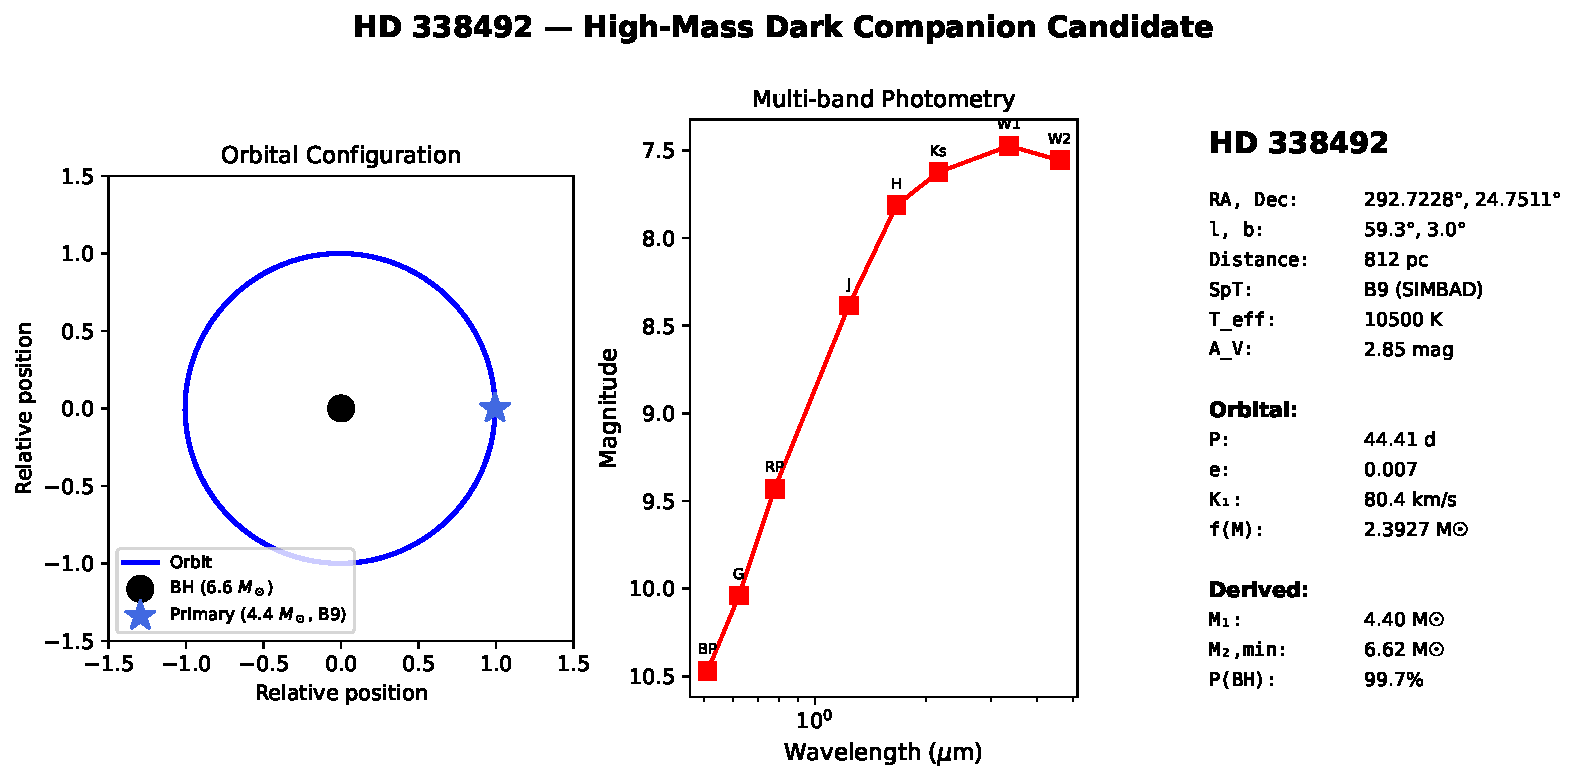
\includegraphics[width=\textwidth]{figures/fig1_system_overview.pdf}
\caption{Overview of the HD~338492 system.  \textit{Left:} Orbital
configuration showing the nearly circular ($e = 0.007$) orbit.
\textit{Centre:} Multi-band observed photometry from Gaia, 2MASS,
and WISE.  \textit{Right:} Summary of key system properties.}
\label{fig:overview}
\end{figure*}

\begin{figure*}
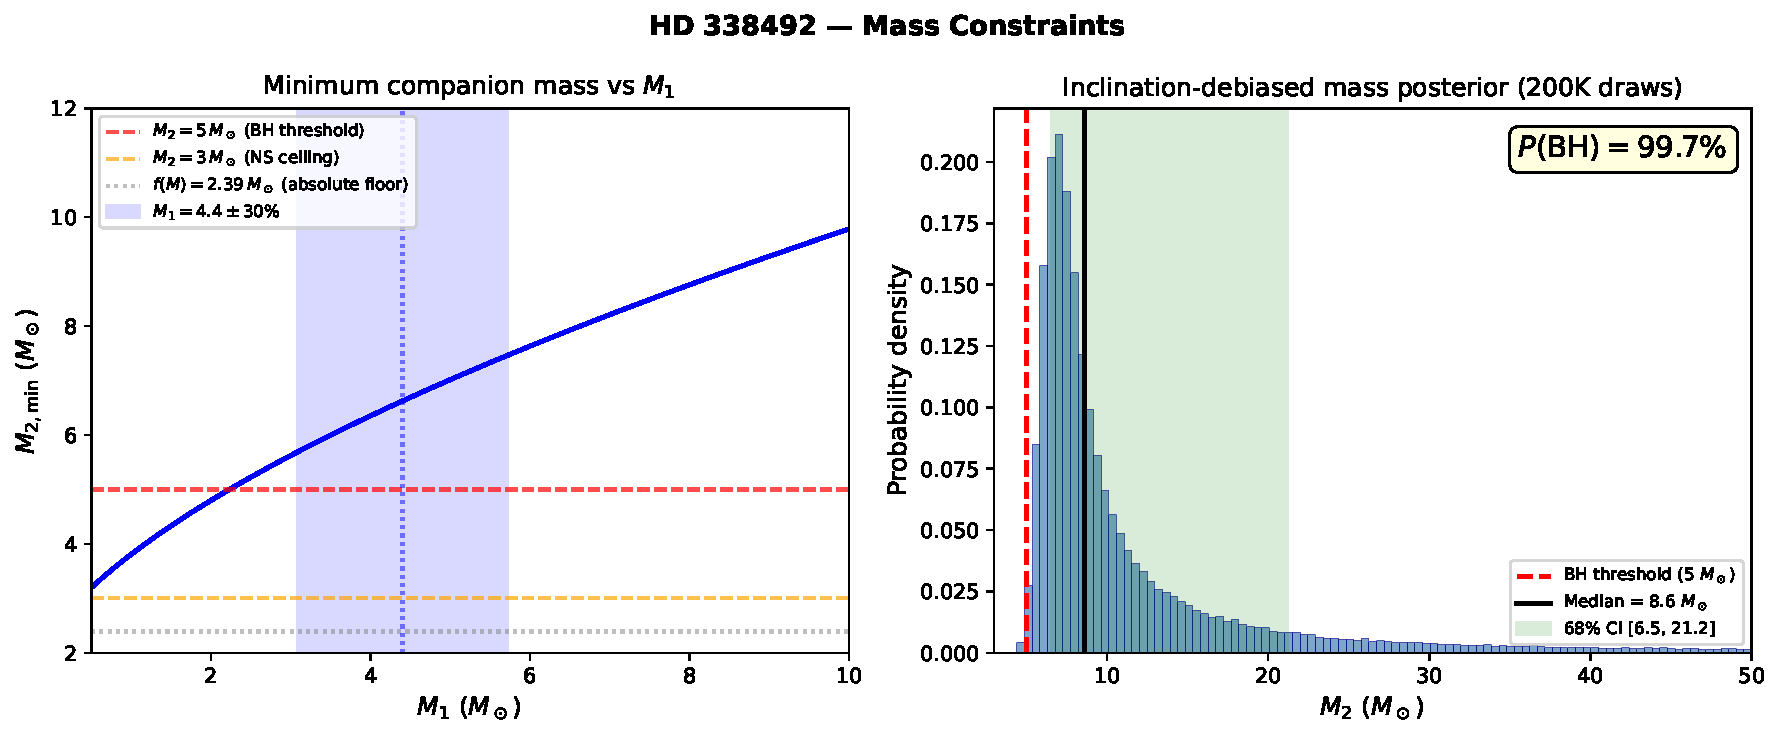
\includegraphics[width=\textwidth]{figures/fig_mass_posterior.pdf}
\caption{\textit{Left:} Minimum companion mass $M_{2,\min}$ as a
function of assumed primary mass $M_1$.  The dashed lines mark the
adopted $M_1 = 4.40\,\Msun$ and the resulting
$M_{2,\min} = 6.62\,\Msun$.  \textit{Bottom:} Monte~Carlo
posterior distribution of $M_2$ from 200\,000 draws with isotropic
inclination and log-normal $M_1$ priors.  The shaded blue region
marks $M_2 > 5\,\Msun$ (BH regime); the integrated probability is
$P(\text{BH}) = 99.7$~per~cent.}
\label{fig:posterior}
\end{figure*}

\begin{figure*}
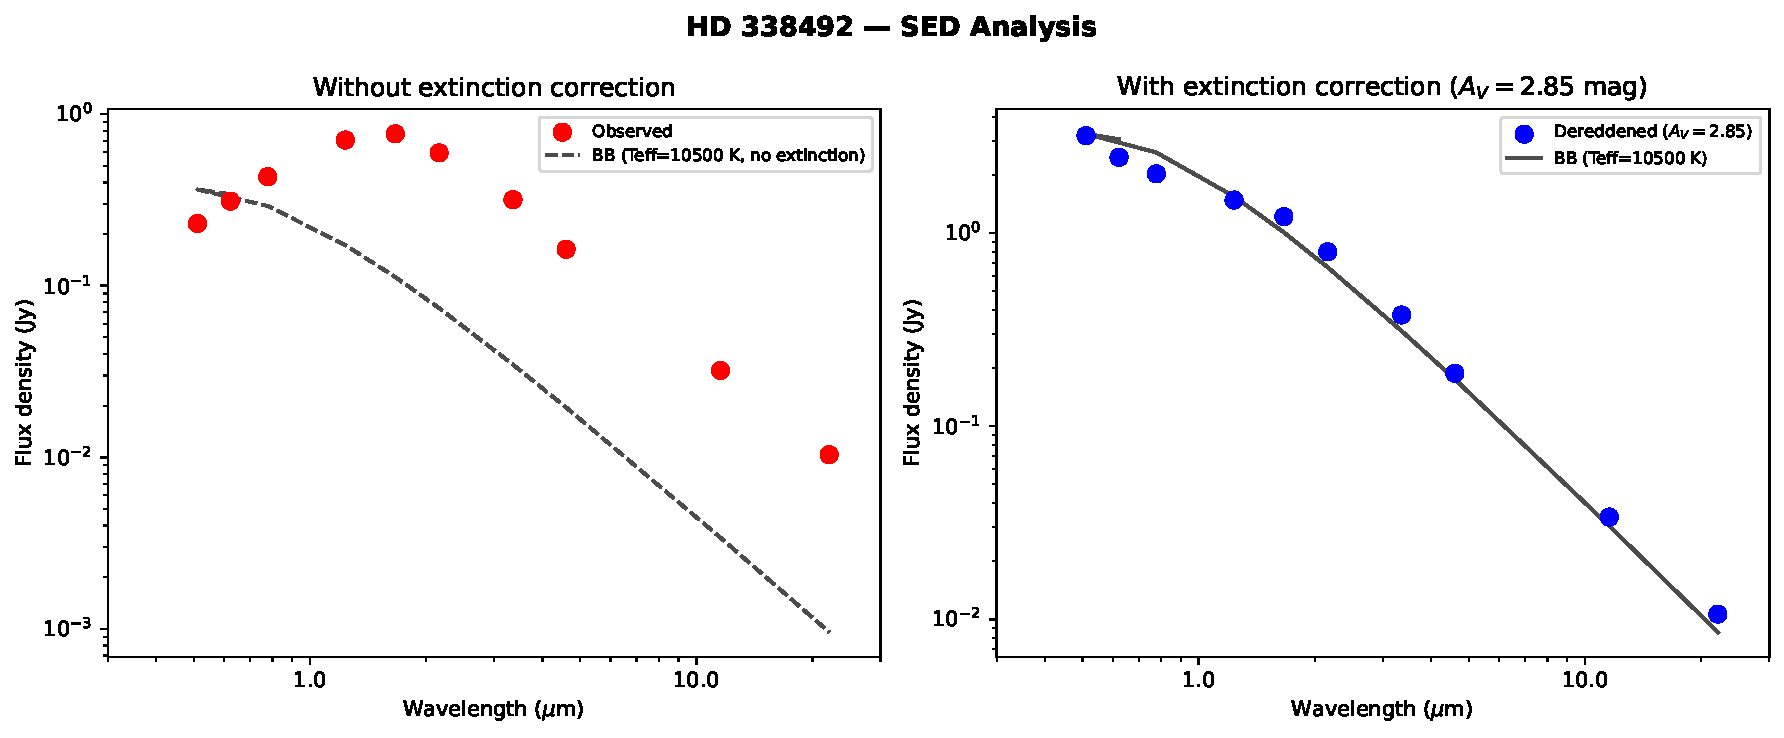
\includegraphics[width=\textwidth]{figures/fig_sed_extinction.pdf}
\caption{Spectral energy distribution of HD~338492.  \textit{Top:}
Observed photometry compared to a 10\,500\,K blackbody --- the
SED is strongly reddened ($\chi^2 \approx 285$).  \textit{Bottom:}
Dereddened photometry ($A_V = 2.85$) compared to the same model ---
$\chi^2 \approx 14$, a 20-fold improvement.  No secondary SED
component is required.}
\label{fig:sed}
\end{figure*}

\begin{figure*}
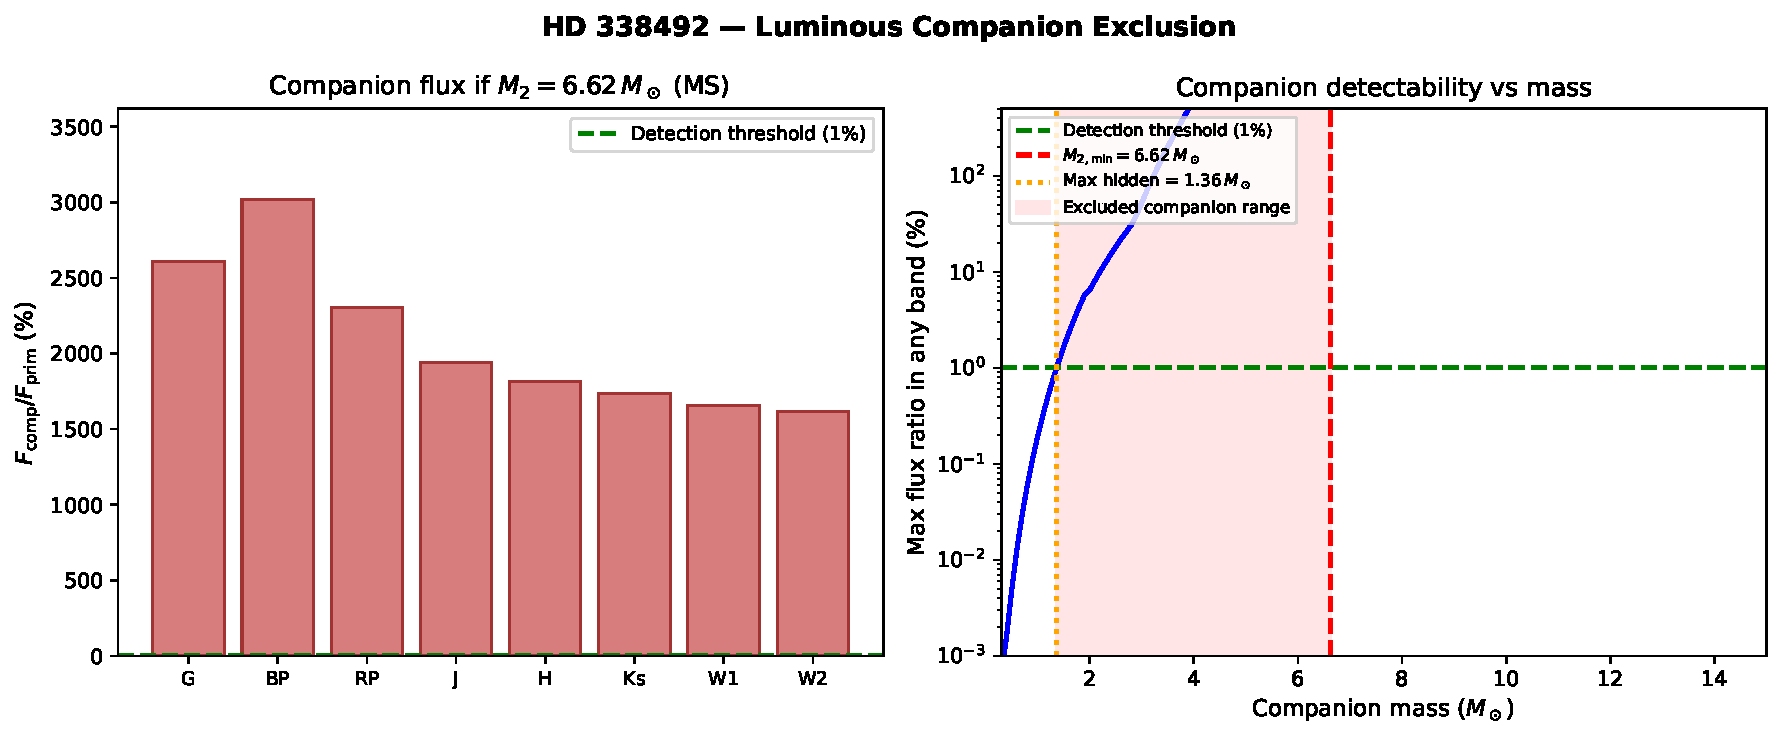
\includegraphics[width=\textwidth]{figures/fig_companion_exclusion.pdf}
\caption{\textit{Left:} Expected companion-to-primary flux ratio
in each photometric band for a hypothetical $6.62\,\Msun$ MS
companion.  All bands exceed the 1~per~cent detection threshold.
\textit{Right:} Maximum flux ratio as a function of companion mass.
The detectable mass threshold is $\sim$\,$1.4\,\Msun$, far below
$M_{2,\min} = 6.62\,\Msun$.}
\label{fig:companion}
\end{figure*}

\begin{figure*}
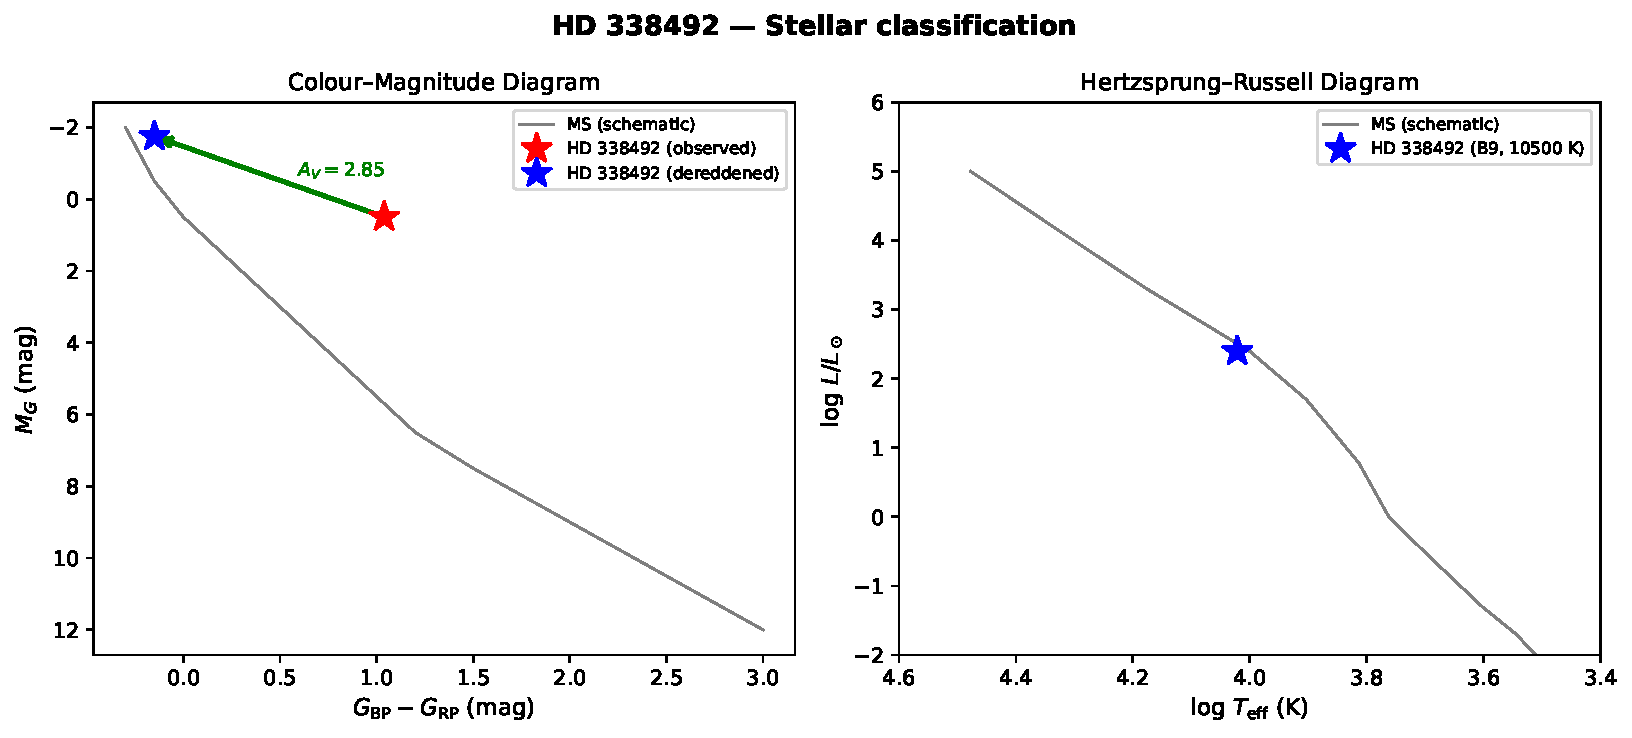
\includegraphics[width=\textwidth]{figures/fig5_cmd_hrd.pdf}
\caption{\textit{Left:} Colour--magnitude diagram showing
HD~338492 before (red) and after (blue) extinction correction.
The green arrow indicates the reddening vector ($A_V = 2.85$).
\textit{Right:} Hertzsprung--Russell diagram placement.  The
dereddened position is consistent with a B9 main-sequence star
of $\sim$\,$4.4\,\Msun$.}
\label{fig:cmd_hrd}
\end{figure*}

\begin{figure*}
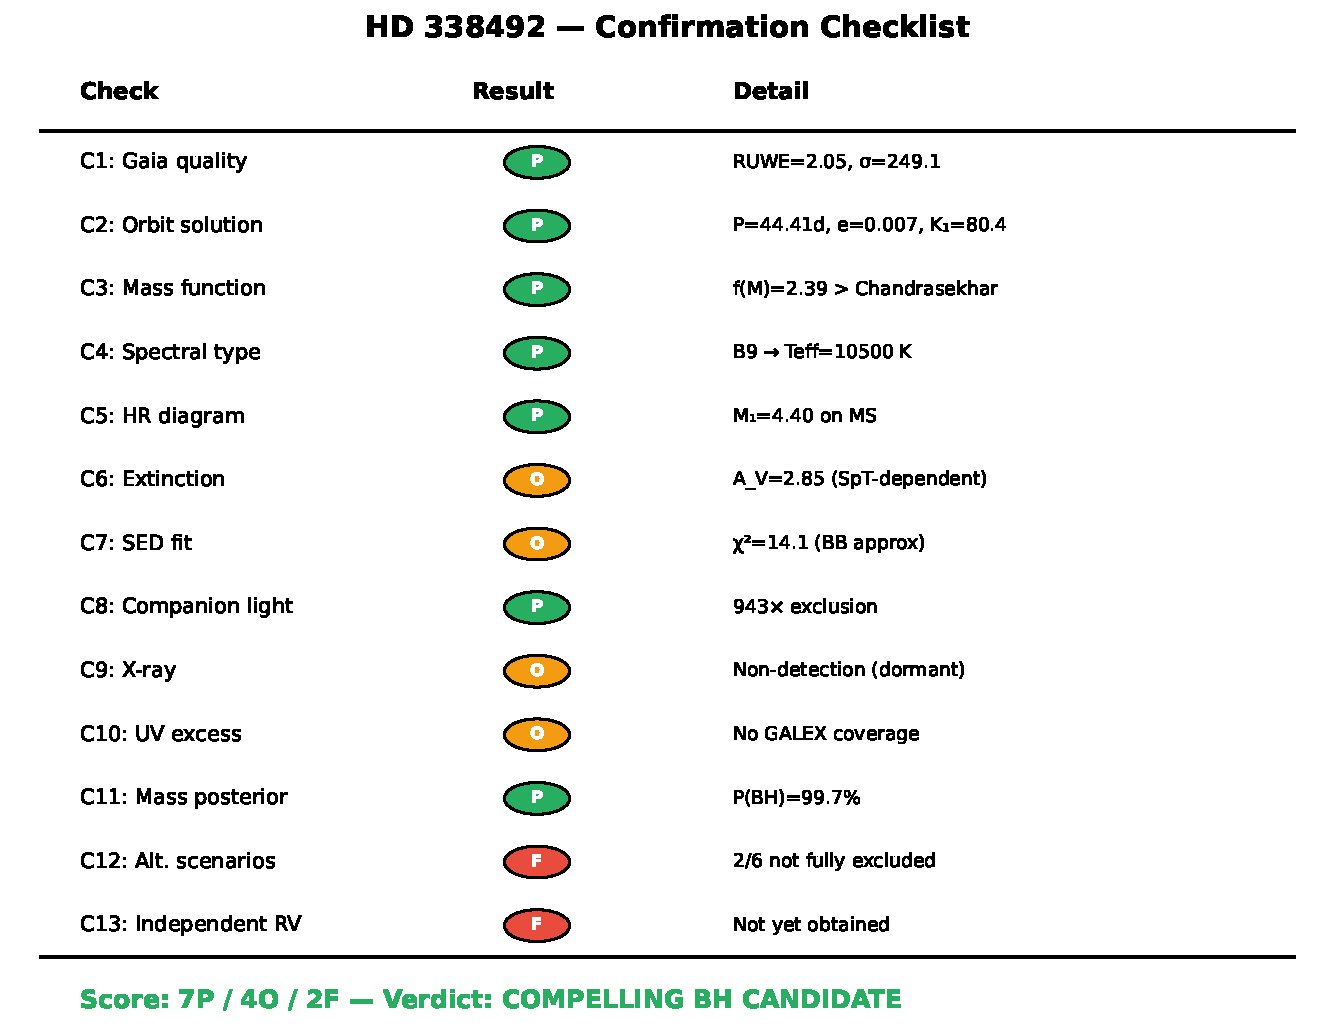
\includegraphics[width=0.85\textwidth]{figures/fig6_confirmation_checklist.pdf}
\caption{Confirmation checklist for HD~338492, showing the outcome
of each diagnostic test.  Green circles indicate PASS, orange
indicates OPEN (inconclusive), red indicates FAIL (not yet
satisfied).  The system scores 7P/4O/2F ---
a ``compelling'' BH candidate requiring follow-up to close the
two remaining failures (independent RV and full scenario exclusion).}
\label{fig:checklist}
\end{figure*}

\label{lastpage}
\end{document}
